\documentclass[a4paper]{article}

\usepackage[margin=3cm]{geometry}
\usepackage{hyperref}
\usepackage{amsmath}
\usepackage{tikz}
\usetikzlibrary{matrix,shapes,positioning,fit,decorations.pathreplacing,arrows,calc}
\usepackage{graphicx}
\usepackage{cleveref}
\usepackage{tabularx}
\usepackage{booktabs}
\usepackage{subcaption}
 \usepackage[doi=true,
 url=false,
 sorting=ydnt,
 maxnames=10,
 backend=biber,
 isbn=false,
 giveninits=true,
 defernumbers=true]{biblatex}
\usepackage{minted}


\bibliography{papers.bib}


\title{Performance analysis and optimisation of matrix-matrix multiplication}

\author{Lawrence Mitchell\thanks{lawrence.mitchell@durham.ac.uk}}

\begin{document}
\maketitle

This assignment is to be completed and handed in via DUO. 
For deadlines, please consult DUO and the level handbook.

\section{Introduction}
\label{sec:introduction}
Matrix-matrix multiplication is at the core of much of scientific
computing.  Despite many years of research, there are still open
questions about the most efficient implementation mechanism.  In this
coursework you will develop code, and optimisation approaches for this
problem.

\section{Level 4 students only}
\label{sec:level-4-students}

\subsection{The BLIS approach to matrix-matrix multiplication}
\label{sec:blis}

When we compare the performance of the optimised matrix-matrix
multiplication presented in the lectures with that provided by a
well-tuned BLAS library (for example Intel's MKL, ATLAS, or OpenBLAS),
we see that there is still a large performance gap.  A general
approach for optimising matrix-matrix multiplication that achieves
close to machine peak was developed by Kazushigo Goto in the early
2000s.  It has subsequently been further developed by Robert van der
Geijn and co-workers in the BLIS (BLAS-like Library Instantiation
Software) framework.

The idea they use is a nested sequence of loops that effectively block
for all levels of the memory hierarchy.  At the very inner-most loop
is a ``microkernel'' that must be tuned to each architecture.

\subsection{Task specification}
\label{sec:task-l4}
Your goal is to implement the BLIS approach for dense matrix-matrix
multiplication.  This is described in two papers, \textcite{Goto:2008}
and \textcite{Zee:2015}.  Since this is such a well-studied problem,
you will no doubt also find more didatic expositions.  You can of
course reference and use these where appropriate, as long as you
\emph{fully acknowledge} them in your submission.

You should evaluate your implementation for its performance, and
provide a summary thereof on a range of problem sizes.  In doing so,
you may wish to compare your results to those provided by an optimised
BLAS implementation, but your solution \emph{must not use code from
  any BLAS library}.  This latter requirement should be interpreted
liberally: you must write the code for the matrix-matrix
multiplication routine yourself, rather than calling out to a library
implementation (even if that library does not have BLAS in its name!).

\subsection{Program specification}
\label{sec:program-l4}
You are provided with a skeleton project written in the C programming
language, along with a \texttt{Makefile} for building the project.
This code is available via DUO and also on github at
\url{https://github.com/wence-/ccs-l4-coursework-2018}.  Bugfixes will
be deployed faster to the latter than the former!

This project provides a simple harness, as well as a naive (triple loop)
implementation of matrix-matrix multiplication.  The project contains
the following files:
\begin{itemize}
\item \texttt{Makefile} builds and runs some simple checks and
  benchmarks.  Type \texttt{make help} to see the targets.
\item \texttt{gemm.c} The main test harness, you should not have to
  edit this unless you wish to change the benchmarking that you do.
\item \texttt{basic-gemm.c} A basic implementation of matrix-matrix
  multiplication.  You should not have to edit this.
\item \texttt{optimised-gemm.c} A stub in which you should implement
  your optimised version.  To begin, this just calls the basic
  implementation.
\item \texttt{plot-benchmarks.py} An example matplotlib script for simple
  plotting of the benchmark results.
\end{itemize}

The signature of the multiplication function you need to implement is:
\begin{minted}{c}
void (*gemm_fn_t)(int m, int n, int k,
                  const double *a, int lda,
                  const double *b, int ldb,
                  double *c, int ldc);
\end{minted}
Where \verb~a~ is an $m\times k$ matrix with leading dimension
\verb~lda~, \verb~b~ is a $k \times n$ matrix with leading dimension
\verb~ldb~, and \verb~c~ is an $m \times n$ matrix with leading
dimension \verb~ldc~.  The data layout and meaning of the
\emph{leading dimension} are described in \cref{sec:data-layout}.

For the purposes of your performance study, you may wish to modify the
benchmarking.  For example, benchmarking multiplication for non-square
matrices, larger matrices, or to extract more information.

\subsubsection{Data layout}
\label{sec:data-layout}
For historical reasons (Fortran), the default for BLAS routines is to
assume all matrices are in \emph{column major} ordering.  The skeleton
code use this layout too, as should your solution.  It turns out
(for tiling and blocking purposes) that it makes most sense to
describe the size of the matrix with three numbers:
\begin{enumerate}
\item $m$: the number of rows;
\item $n$: the number of columns;
\item $\operatorname{ldX}$: the \emph{leading dimension}.
\end{enumerate}
All matrices are allocated as contiguous, one-dimensional arrays,
where the column index has stride-1 access (moving down the column,
the data is contiguous), and the row index has
stride-$\operatorname{ldX}$ access.  This is illustrated in
\cref{fig:matrix-layout-full} for a $5\times 4$ matrix.
\begin{figure}[htbp]
  \begin{subfigure}[l]{0.475\textwidth}
    \centering
    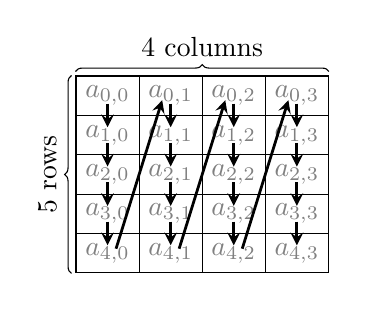
\begin{tikzpicture} [nodes in empty cells,
      nodes={minimum width=0.5cm, minimum height=0.5cm},
      row sep=-\pgflinewidth, column sep=-\pgflinewidth]
      border/.style={draw}

      \matrix(matrix)[matrix of nodes,
      nodes={draw, text=gray}]
      {
        $a_{0,0}$  & $a_{0,1}$  & $a_{0,2}$  & $a_{0,3}$  \\
        $a_{1,0}$  & $a_{1,1}$  & $a_{1,2}$  & $a_{1,3}$  \\
        $a_{2,0}$  & $a_{2,1}$  & $a_{2,2}$  & $a_{2,3}$  \\
        $a_{3,0}$  & $a_{3,1}$  & $a_{3,2}$  & $a_{3,3}$  \\
        $a_{4,0}$  & $a_{4,1}$  & $a_{4,2}$  & $a_{4,3}$  \\
      };
      \draw[decoration={brace,raise=0.05cm},decorate] (matrix-1-1.north west)
      -- (matrix-1-4.north east) node [pos=0.5, anchor=south, yshift=0.1cm] {4 columns};
      \draw[decoration={brace,raise=0.05cm},decorate] (matrix-5-1.south west)
      -- (matrix-1-1.north west) node [pos=0.5, anchor=south, rotate=90,
      yshift=0.1cm] {5 rows};
      \foreach \c in {1, 2, 3, 4} {
        \foreach \i/\j in {1/2, 2/3, 3/4, 4/5} {
          \draw[-stealth, line width=1] ($(matrix-\i-\c.center) + (0, -0.1)$)
          -- ($(matrix-\j-\c.center) + (0, +0.1)$);
        };
      };
      \foreach \i/\j in {5-1/1-2, 5-2/1-3, 5-3/1-4} {
        \draw[-stealth, line width=1] ($(matrix-\i.north east) + (-0.3, -0.2)$)
        -- ($(matrix-\j.south west) + (0.3, 0.2)$);
      };
    \end{tikzpicture}
    \caption{Data layout for a $5 \times 4$ matrix.  It has $m = 5$
      rows, $n = 4$ columns and leading dimension $\operatorname{ldX}
      = 5$.\label{fig:matrix-layout-full}}
  \end{subfigure}
  \hspace{1em}
  \begin{subfigure}[r]{0.475\textwidth}
    \centering
    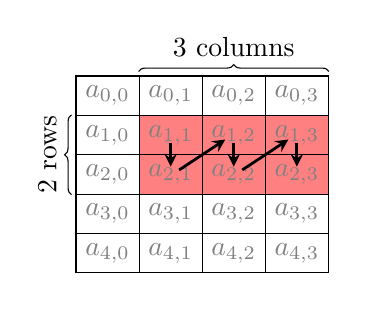
\begin{tikzpicture} [nodes in empty cells,
      nodes={minimum width=0.5cm, minimum height=0.5cm},
      row sep=-\pgflinewidth, column sep=-\pgflinewidth]
      border/.style={draw}

      \matrix(matrix)[matrix of nodes,
      nodes={draw, text=gray}]
      {
        $a_{0,0}$ & $a_{0,1}$                 & $a_{0,2}$                 & $a_{0,3}$                 \\
        $a_{1,0}$ & |[fill=red!50]|$a_{1,1}$  & |[fill=red!50]| $a_{1,2}$ & |[fill=red!50]| $a_{1,3}$ \\
        $a_{2,0}$ & |[fill=red!50]| $a_{2,1}$ & |[fill=red!50]| $a_{2,2}$ & |[fill=red!50]| $a_{2,3}$ \\
        $a_{3,0}$ & $a_{3,1}$                 & $a_{3,2}$                 & $a_{3,3}$                 \\
        $a_{4,0}$ & $a_{4,1}$                 & $a_{4,2}$                 & $a_{4,3}$                 \\
      };
      \draw[decoration={brace,raise=0.05cm},decorate] (matrix-1-2.north west)
      -- (matrix-1-4.north east) node [pos=0.5, anchor=south, yshift=0.1cm] {3 columns};
      \draw[decoration={brace,raise=0.05cm},decorate] (matrix-3-1.south west)
      -- (matrix-2-1.north west) node [pos=0.5, anchor=south, rotate=90,
      yshift=0.1cm] {2 rows};
      \foreach \c in {2, 3, 4} {
        \foreach \i/\j in {2/3} {
          \draw[-stealth, line width=1] ($(matrix-\i-\c.center) + (0, -0.1)$)
          -- ($(matrix-\j-\c.center) + (0, +0.1)$);
        };
      };
      \foreach \i/\j in {3-2/2-3, 3-3/2-4} {
        \draw[-stealth, line width=1] ($(matrix-\i.north east) + (-0.3, -0.2)$)
        -- ($(matrix-\j.south west) + (0.3, 0.2)$);
      };
    \end{tikzpicture}
    \caption{Selecting a $2 \times 3$ submatrix.  Achieved by passing
      a pointer to $a_{1,1}$ and providing $m = 2$, $n = 3$ and
      $\operatorname{ldX} = 5$.\label{fig:matrix-layout-slice}}
  \end{subfigure}
  \caption{Column major data layout, arrows show the unit stride indexing directions}
  \label{fig:matrix-layout}
\end{figure}
The utility of the leading dimension can be observed when we want to
address a small sub-matrix without copying data.  Consider allocating
a zeroed $5 \times 4$ matrix:
\begin{minted}{c}
int m = 5;
int n = 4;
double *a = calloc(m*n, sizeof(double));
\end{minted}
Then let us suppose that we wish to set a $2 \times 3$ subblock
starting at row 1, column 1 to the value 1.  This can be achieved by
referencing a pointer to the $a_{1, 1}$ entry, and providing
appropriate size and leading dimension arguments:
\begin{minted}[mathescape=true]{c}
int lda = m;
/* pointer to $a_{1,1}$. */
double *sub = &a[1*lda + 1];
for (int i = 0; i < 3; i++) {
  for (int j = 0; j < 2; j++) {
    sub[i*lda + j] = 1;
  }
}
\end{minted}
The slice being selected is shown in \cref{fig:matrix-layout-slice}.

This mechanism is used in the skeleton code to describe matrix shapes,
and you will find it very useful when implementing your optimised
code, since you can abstract away most of the index manipulations
required in the algorithm by just passing pointers to the relevant
part of the matrix.

\subsubsection{Program requirements}
\label{sec:requirements-l4}
To facilitate easy testing, your submission must meet the following
functional requirements:
\begin{enumerate}
\item Your submission must compile and run on the lab PCs under Linux.
\item Your submission should build an executable with \texttt{make gemm}.
\item Your submission should \emph{at least} pass \texttt{make check}.
  Note that this is a very weak test, it will also be tested for other
  parameter values.
\end{enumerate}

In your implementation, you may restrict yourself to:
\begin{itemize}
\item Single thread performance.
\item Double precision, square matrices.
\end{itemize}
You may find that it is no more difficult to develop an implementation
for general, rectangular matrices than for square ones.


\section{Marks}
\label{sec:marks}

There are in total 100 marks for the coursework, they
will be awarded as follows:

\begin{center}
  \renewcommand\tabularxcolumn[1]{m{#1}}
  \begin{tabularx}{0.9\linewidth}{Xcc}
    \toprule
    Descriptor & Marks (Level 3) & Marks (Level 4) 
    \\
    \midrule
    Accuracy of performance analysis in report & 5 & 10 \\
    Quality of writing                         & 5 & 5 \\
    \midrule
    Tested for three different, unseen matrices (applies to code from \cref{sec:both}): \\
    Correct result & $3 \times 10 $  & $3 \times 5 $ \\
    Single-thread performance & $3 \times 10 $  & $3 \times 5 $ \\
    Scalability & $3 \times 10 $  & $3 \times 5 $ \\
    \midrule
    Description of BLIS realisation & does not apply  & 10 \\
    Performance $>50\%$ peak (for all matrix sizes) & does not apply & 10\\
    Performance $>80\%$ peak (for all matrix sizes) & does not apply & 10\\
    Implementation working for non-square matrices & does not apply & 5\\
    Performance better than OpenBLAS implementation (for any size $>64\times 64$) & does not apply & 5\\
    \midrule
    Total                                               & 100 & 100       \\
    \bottomrule
  \end{tabularx}
\end{center}

\subsection{Submission: Level 3 students}
\label{sec:submission-level-3}

Level 3 students must submit the following via DUO.
\begin{itemize}
\item \textbf{Brief report: max 750 words (it can be shorter!)}
  detailing your approach to the problem and evaluating the
  performance of your solution (includes performance analysis).
  Provide any illustrative figures or tables of the performance data
  that you collected, demonstrating that you have achieved the goal of
  a fast sparse matrix-matrix multiply.  The word limit is for prose text:
  any titles, captions, tables, references, and graphs do not count
  towards the total word count.

  \textbf{This document \emph{must} be submitted as a PDF}.

\item \textbf{Full program source code} for your solution to
  \cref{sec:both}, as a tarball of all the relevant project files.
  Compilation and usage through the command line must be the same as
  for the provided code template.  Ensure that your submission meets
  the functional requirements of \cref{sec:requirements-l3}.
\end{itemize}


\subsection{Submission: Level 4 students}
\label{sec:submission-level-4}

Level 4 students must submit the following via DUO.
\begin{itemize}
\item \textbf{Brief report: max 1000 words (it can be shorter!)}
  detailing your approach to the problem and evaluating the
  performance of your solution (includes performance analysis).
  Provide any illustrative figures or tables of the performance data
  that you collected, demonstrating that you have achieved the goal of
  a fast sparse matrix-matrix multiply.

  This report should also include a description of your implementation
  of the BLIS scheme for \cref{sec:level-4-students}.

  The word limit is for prose text: any titles, captions, tables,
  references, and graphs do not count towards the total word count.

  \textbf{This document \emph{must} be submitted as a PDF}.

\item \textbf{Full program source code} for your solution to
  \cref{sec:both}, as a tarball of all the relevant project files.
  Compilation and usage through the command line must be the same as
  for the provided code template.  Ensure that your submission meets
  the functional requirements of \cref{sec:requirements-l3}.

\item \textbf{Full program source code} for your solution to
  \cref{sec:level-4-students}.  This should be provided as a tarball
  of all the relevant project files.  Ensure that your submission
  meets the functional requirements of \cref{sec:requirements-l4}.
\end{itemize}
\printbibliography

\end{document}
